\section{Práctica propuesta}
\label{sec:practica}

Se presenta a continuación el planteamiento de la práctica a realizar por los alumnos de la asignatura de Sistemas Eléctricos II.

\newpage

\section*{Diseño y optimización de una lanzadera electromagnética}

\subsection*{Objetivo}

El objetivo de esta práctica es que los estudiantes diseñen y construyan la bobina de una lanzadera electromagnética optimizando su geometría y alimentación para lograr la mayor fuerza de atracción magnética y por ende velocidad del proyectil. Se deberán aplicar conocimientos teórico-prácticos de electromagnetismo en tres entornos: MATLAB\textsuperscript{\textregistered}, ANSYS Maxwell\textsuperscript{\textregistered} y laboratorio.

\subsection*{Marco teórico}

En esta sección se desarrollarán los principios teóricos que permiten el funcionamiento de las lanzaderas electromagnéticas. Para entender estos principios, es esencial comprender los fundamentos del electromagnetismo, el concepto de bobina y su papel en la generación de campos magnéticos.

El comportamiento de las ondas electromagnéticas está definido por las ecuaciones de Maxwell, descritas a continuación:
\begin{figure}[H]
    \centering
    \[
    \vec{\nabla}\cdot \vec{E}= \frac{\rho}{\epsilon_0}~~~~~~\vec{\nabla}\cdot \vec{B}= 0
    \]
    \[
    \vec{\nabla}\times\vec{E}=-\frac{\partial\vec{B}}{\partial t}~~~~~~\vec{\nabla}\times \vec{B}=\mu_0\vec{J}+\mu_0\epsilon_0\frac{\partial \vec{E}}{\partial t}
    \]
\end{figure}

En el caso de esta práctica, la ley de mayor interés es la de Ampère. Esta es la ley que define la relación entre un campo magnético y uno eléctrico, y partir de su forma diferencial expresada en las ecuaciones de Maxwell, se puede desarrollar la ley integral de Ampère como:

\begin{quote}
    "La integral de línea del campo magnético \(\mathbf{B}\) alrededor de un lazo cerrado es igual a \(\mu_0\) multiplicado por la corriente total \(I_{enc}\) que pasa a través de cualquier superficie delimitada por el lazo. Matemáticamente, esto se expresa como:
    \[
    \oint_{\partial S} \mathbf{B} \cdot d\mathbf{l} = \mu_0 I_{enc}
    \]
    donde \(\mu_0\) es la permeabilidad del vacío."
\end{quote}

Esta ley es esencial porque proporciona el punto de partida de la práctica. Debido a que el componente principal de una lanzadera es una bobina, desde la ley integral de Ampère se puede deducir la expresión del campo magnético generado por la misma:

\[B=\mu_0\mu_r\frac{NI}{L}\]

\noindent Siendo:\\
\\ \(B\) valor del campo magnético en [T].\\
\(\mu_0\) valor de la permeabilidad del vacío. Constante e igual a \(4\pi*10^{-7}\) [Hm\(^-1\)].\\
\(\mu_r\) valor de la permeabilidad relativa del núcleo de la bobina.\\
\(N\) número de espiras del solenoide.\\
\(I\) corriente de alimentación de la bobina [A].\\
\(L\) longitud de la bobina [m].\\

Todo esto además de la ecuación de campo magnético de Gauss (\(\vec{\nabla}\cdot\vec{B} = 0\)) nos lleva a que el campo magnético alrededor de una bobina tiene la siguiente forma y polaridad:

\begin{figure}[H]
    \centering %\raggedleft \raggedright
    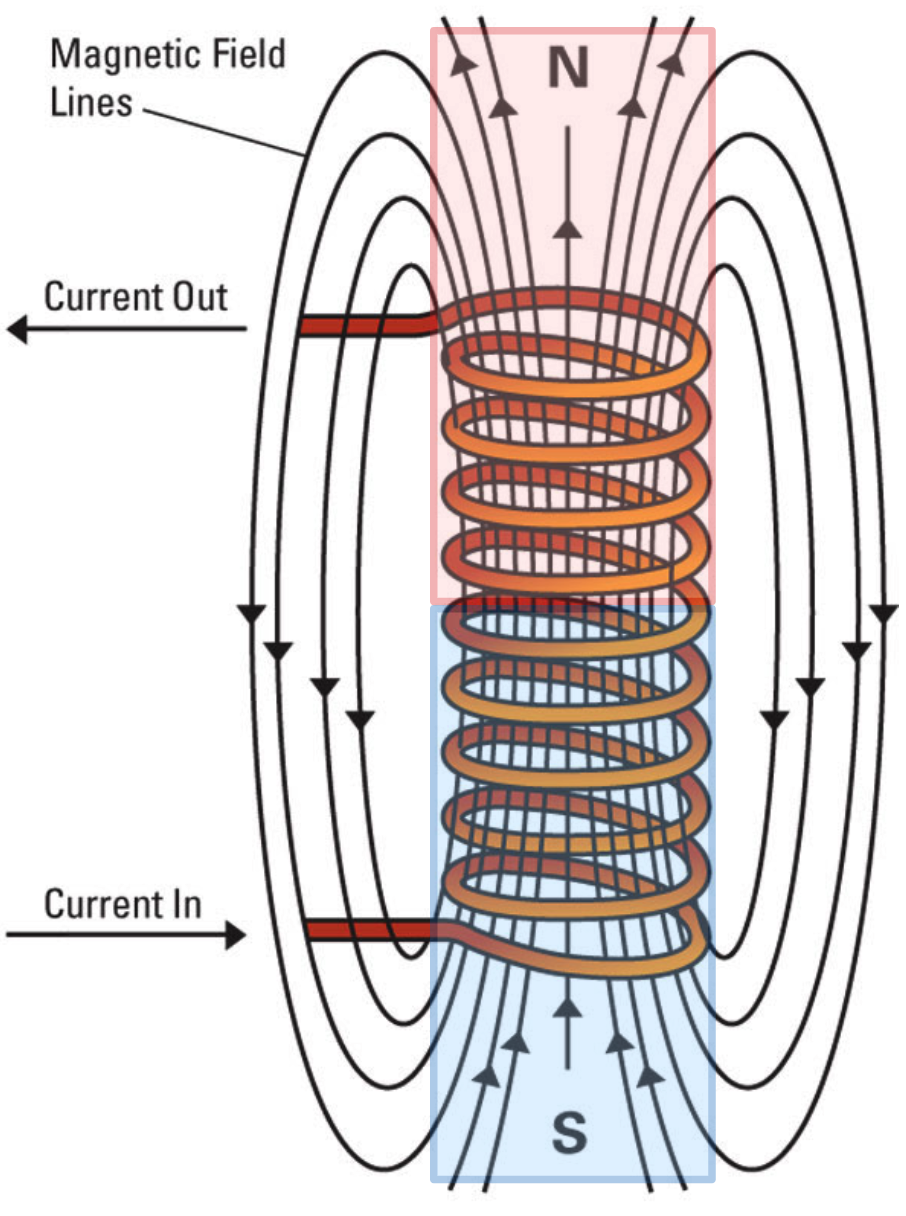
\includegraphics[width=6cm]{FigurasMemoria/electromagnet.png}
    \caption{Visualización del campo magnético de una bobina energizada.}
    \label{fig:electromagnet2} %Para referenciar -> \ref{fig:figNum}
\end{figure}

Por ende, si a la situación que observamos en la figura anterior, le añadimos un elemento de material ferromagnético en uno de los extremos del solenoide, este se verá atraído hasta su centro. Aprovechando este suceso, podemos controlar la alimentación de la bobina para que solamente esté energizada durante el tiempo necesario para atraer el vástago al punto deseado. Una vez que el vástago alcance el centro de la bobina, cortaremos la alimentación para que deje de ser atraído y continúe su movimiento por inercia. El objetivo final de la práctica es predecir cuál va a ser la fuerza ejercida por la bobina sobre el proyectil mediante software, optimizar la geometría para conseguir la mayor densidad energética posible y comprobar las predicciones en el banco de pruebas.

\subsection*{Modelo de la bobina y parámetros iniciales}

El modelo del sistema con el que trabajaremos durante los siguientes apartados consta de las siguientes variables:

\begin{itemize}
    \item \textbf{Parámetros geométricos}:
    \begin{enumerate}[label=\alph*., leftmargin=*, itemindent=1em]
        \item \(r_{cext}\) y \(r_{cint} \): radios exterior e interior de la bobina, respectivamente [m].
        \item \(l_c\): altura de la bobina [m].
        \item \(D_{cu}\): diámetro de la sección del conductor [m].
        \item \(r_{fe}\): radio del vástago [m].
        \item \(l_{fe}\): longitud del vástago [m].
        \item \(k_{disp}\): parámetro multiplicador para obtener la sección de dispersión.
    \end{enumerate}
    \item \textbf{Parámetros eléctricos}:
    \begin{enumerate}[label=\alph*., leftmargin=*, itemindent=1em]
        \item \(N\): número de espiras.
        \item \(V_{cc}\): tensión de alimentación del solenoide [V].
        \item \(\mu_0 = 4\pi*10^{-7}\): permeabilidad del vacío [Hm\(^{-1}\)]. 
        \item \(\mu_{fe}\): permeabilidad relativa del vástago ferromagnético.
    \end{enumerate}
\end{itemize}

\begin{figure}[H]
    \centering 
    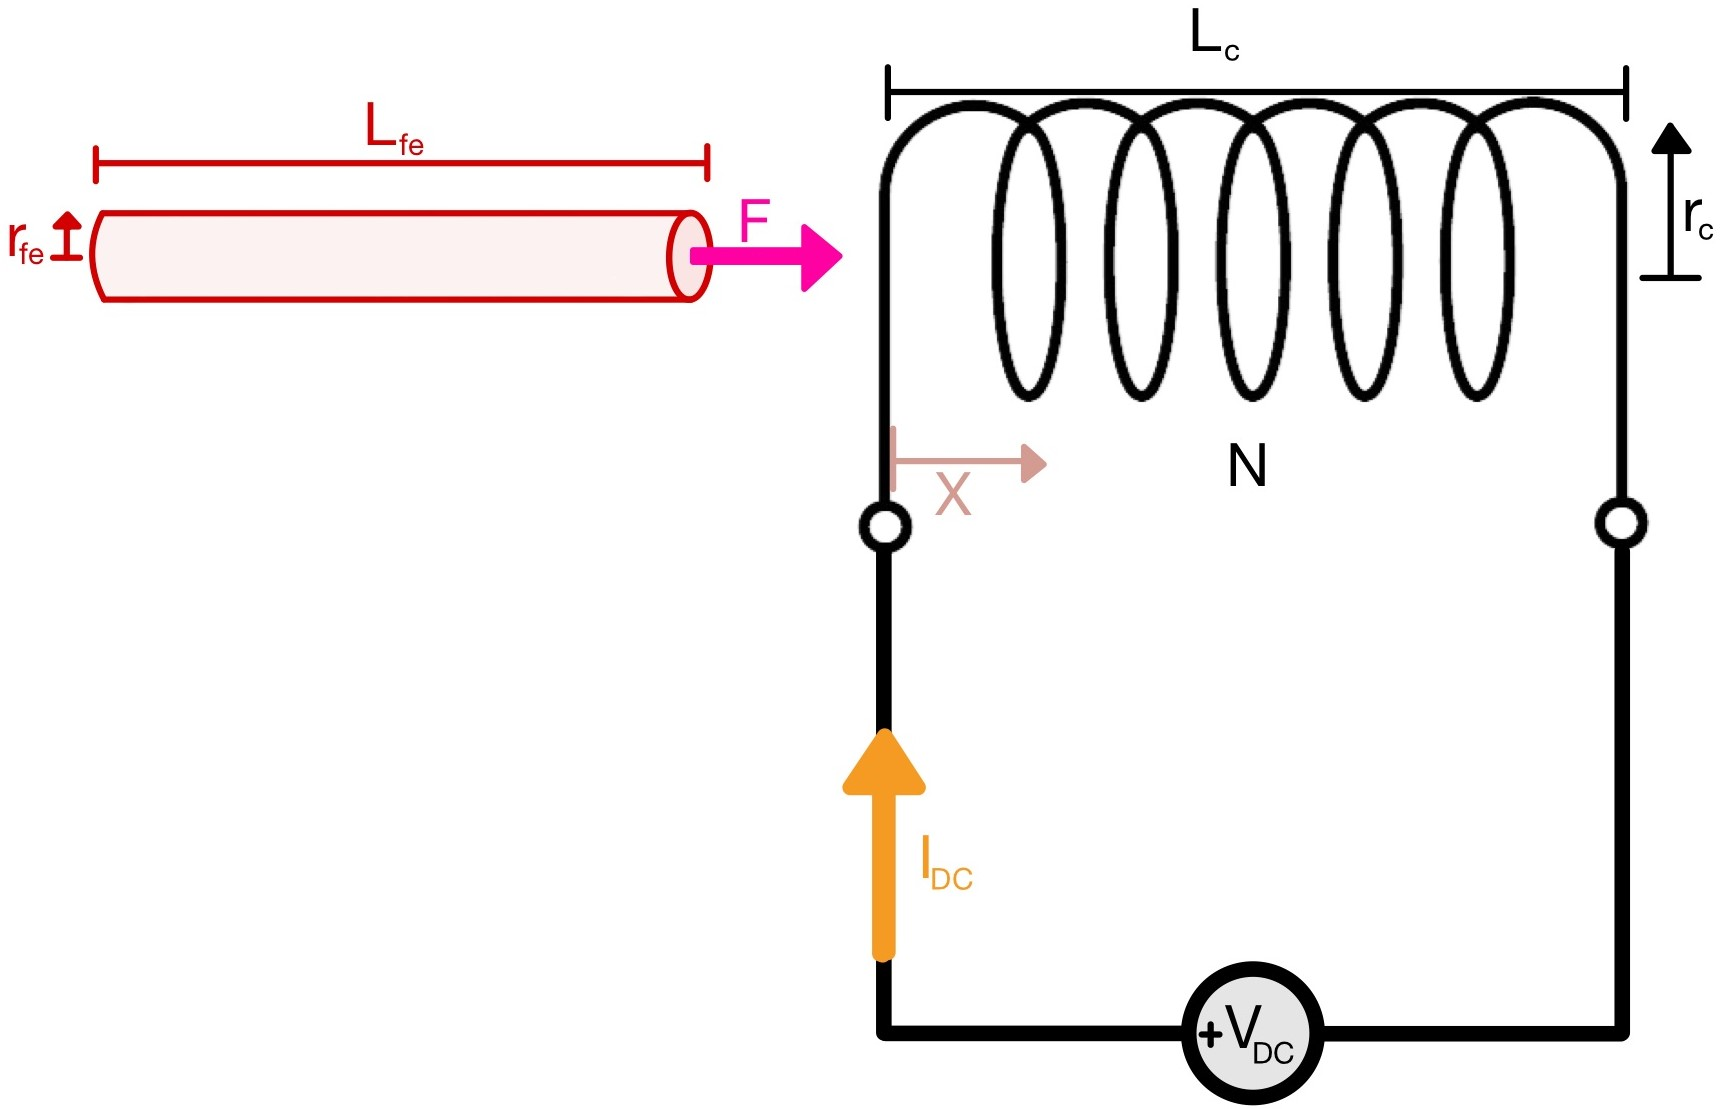
\includegraphics[width=10cm]{FigurasMemoria/esquemaDesTeor.jpg}
    \caption{Esquema geométrico del sistema.}
    \label{fig:esquemaGeomPractica} %Para referenciar -> \ref{fig:figNum}
\end{figure}

El primer paso de esta práctica será elegir la geometría de la bobina inicial sobre la que se realizarán los cálculos de los modelos y las pruebas iniciales. Para ello, se debe rellenar la tabla \ref{tab:bobIniPractica} con valores dentro de los intervalos especificados y teniendo en cuenta las siguientes condiciones:

\begin{itemize}
    \item \(r_{cext} = r_{cint} + \frac{ND_{cu}^2}{l_c}\)
    \item \(r_{cext} \leq 30~\text{mm}\)
    \item \(l_c \leq 133.20~\text{mm}\)
    \item \(l_c \leq l_{fe}\)
    \item \(V_{cc} \leq 30\)V
    \item El valor de \(r_{cint}\) dependerá del cilindro sobre el que se vaya a bobinar el solenoide. Elegirlo del laboratorio y tomar la medida.
\end{itemize}

\begin{table}[H]
    \centering
    \setlength{\tabcolsep}{5pt}
    \renewcommand{\arraystretch}{1.2}
    \begin{tabular}{|c|c|c|c|c|c|c|}
        \hline
        \hbox{} & \textbf{\(D_{cu}\) [mm]} & \textbf{\(l_c\) [mm]} & \textbf{\(r_{fe}\) [mm]} & \textbf{\(l_{fe}\) [mm]} & \textbf{N} & \textbf{\(V_{cc}\) [V]} \\
        \hline
        \textbf{Valor mínimo} & 0,8 & - & - & - & 1 & 1 \\
        \textbf{Valor máximo} & 1,6 & 132,20 & \(r_{cint}-3\) & - & - & 30 \\
        \hline
        \textbf{Valor elegido} &  &  &  &  &  &  \\
        \hline
    \end{tabular}
    \caption{Valores iniciales para la bobina de la lanzadera.}
    \label{tab:bobIniPractica}
\end{table}


\subsection*{Modelo analítico en MATLAB\textsuperscript{\textregistered}}

El objetivo de esta parte es computar el modelo de la figura \ref{fig:esquemaGeomPractica} en MATLAB\textsuperscript{\textregistered} para que devuelva unas gráficas con la evolución de la fuerza de atracción experimentada por el vástago en función de su posición.

Para ello, será necesario realizar el circuito magnético equivalente del sistema. Dicho circuito estará compuesto por las siguientes reluctancias, que deben ser desarrolladas por el alumno:

\[\mathcal{R} = \frac{l_{caract}}{\mu_r\mu_0 S_{efect}}\]

\begin{itemize}
    \item \(\mathcal{R}_{disp~c}\): Será la reluctancia de dispersión de la bobina. No es dependiente de \textit{x}.
    \item \(\mathcal{R}_{Fe}\): Será la reluctancia correspondiente al vástago. No es dependiente de \textit{x}.
    \item \(\mathcal{R}_{\phi}\): Será la reluctancia correspondiente al camino del flujo magnético que abraza todo el sistema. Es dependiente de \textit{x}.
    \item \(\mathcal{R}_{aire~c}\): Será la reluctancia correspondiente al volumen de aire que hay dentro de la bobina. Es dependiente de \textit{x}.
\end{itemize}

Una vez elegidas las longitudes y secciones efectivas de cada una de las reluctancias expresadas, se podrá calcular la inducción magnética según:

\[B = \frac{NI}{\sum\mathcal{R}}\]

Y la expresión de la fuerza de atracción magnética sobre un cuerpo \textit{T} cualquiera es:

\[F_T = \frac{1}{2} \frac{B_T^2*S_{efect~T}}{\mu_0}\]

Teniendo en cuenta que \textit{x} es la posición del extremo del vástago, que su intervalo de interés para la práctica es \(x\in [0, l_c]\) y que el circuito magnético cambia para cada valor de \textit{x}, se pide diseñar el código y rellenar las figuras \ref{fig:grafReluctPractica}, \ref{fig:grafInducPractica} y \ref{fig:grafFuerzaPractica} con los los valores obtenidos. El resultado puede ser algo como:

\begin{figure}[H]
    \centering 
    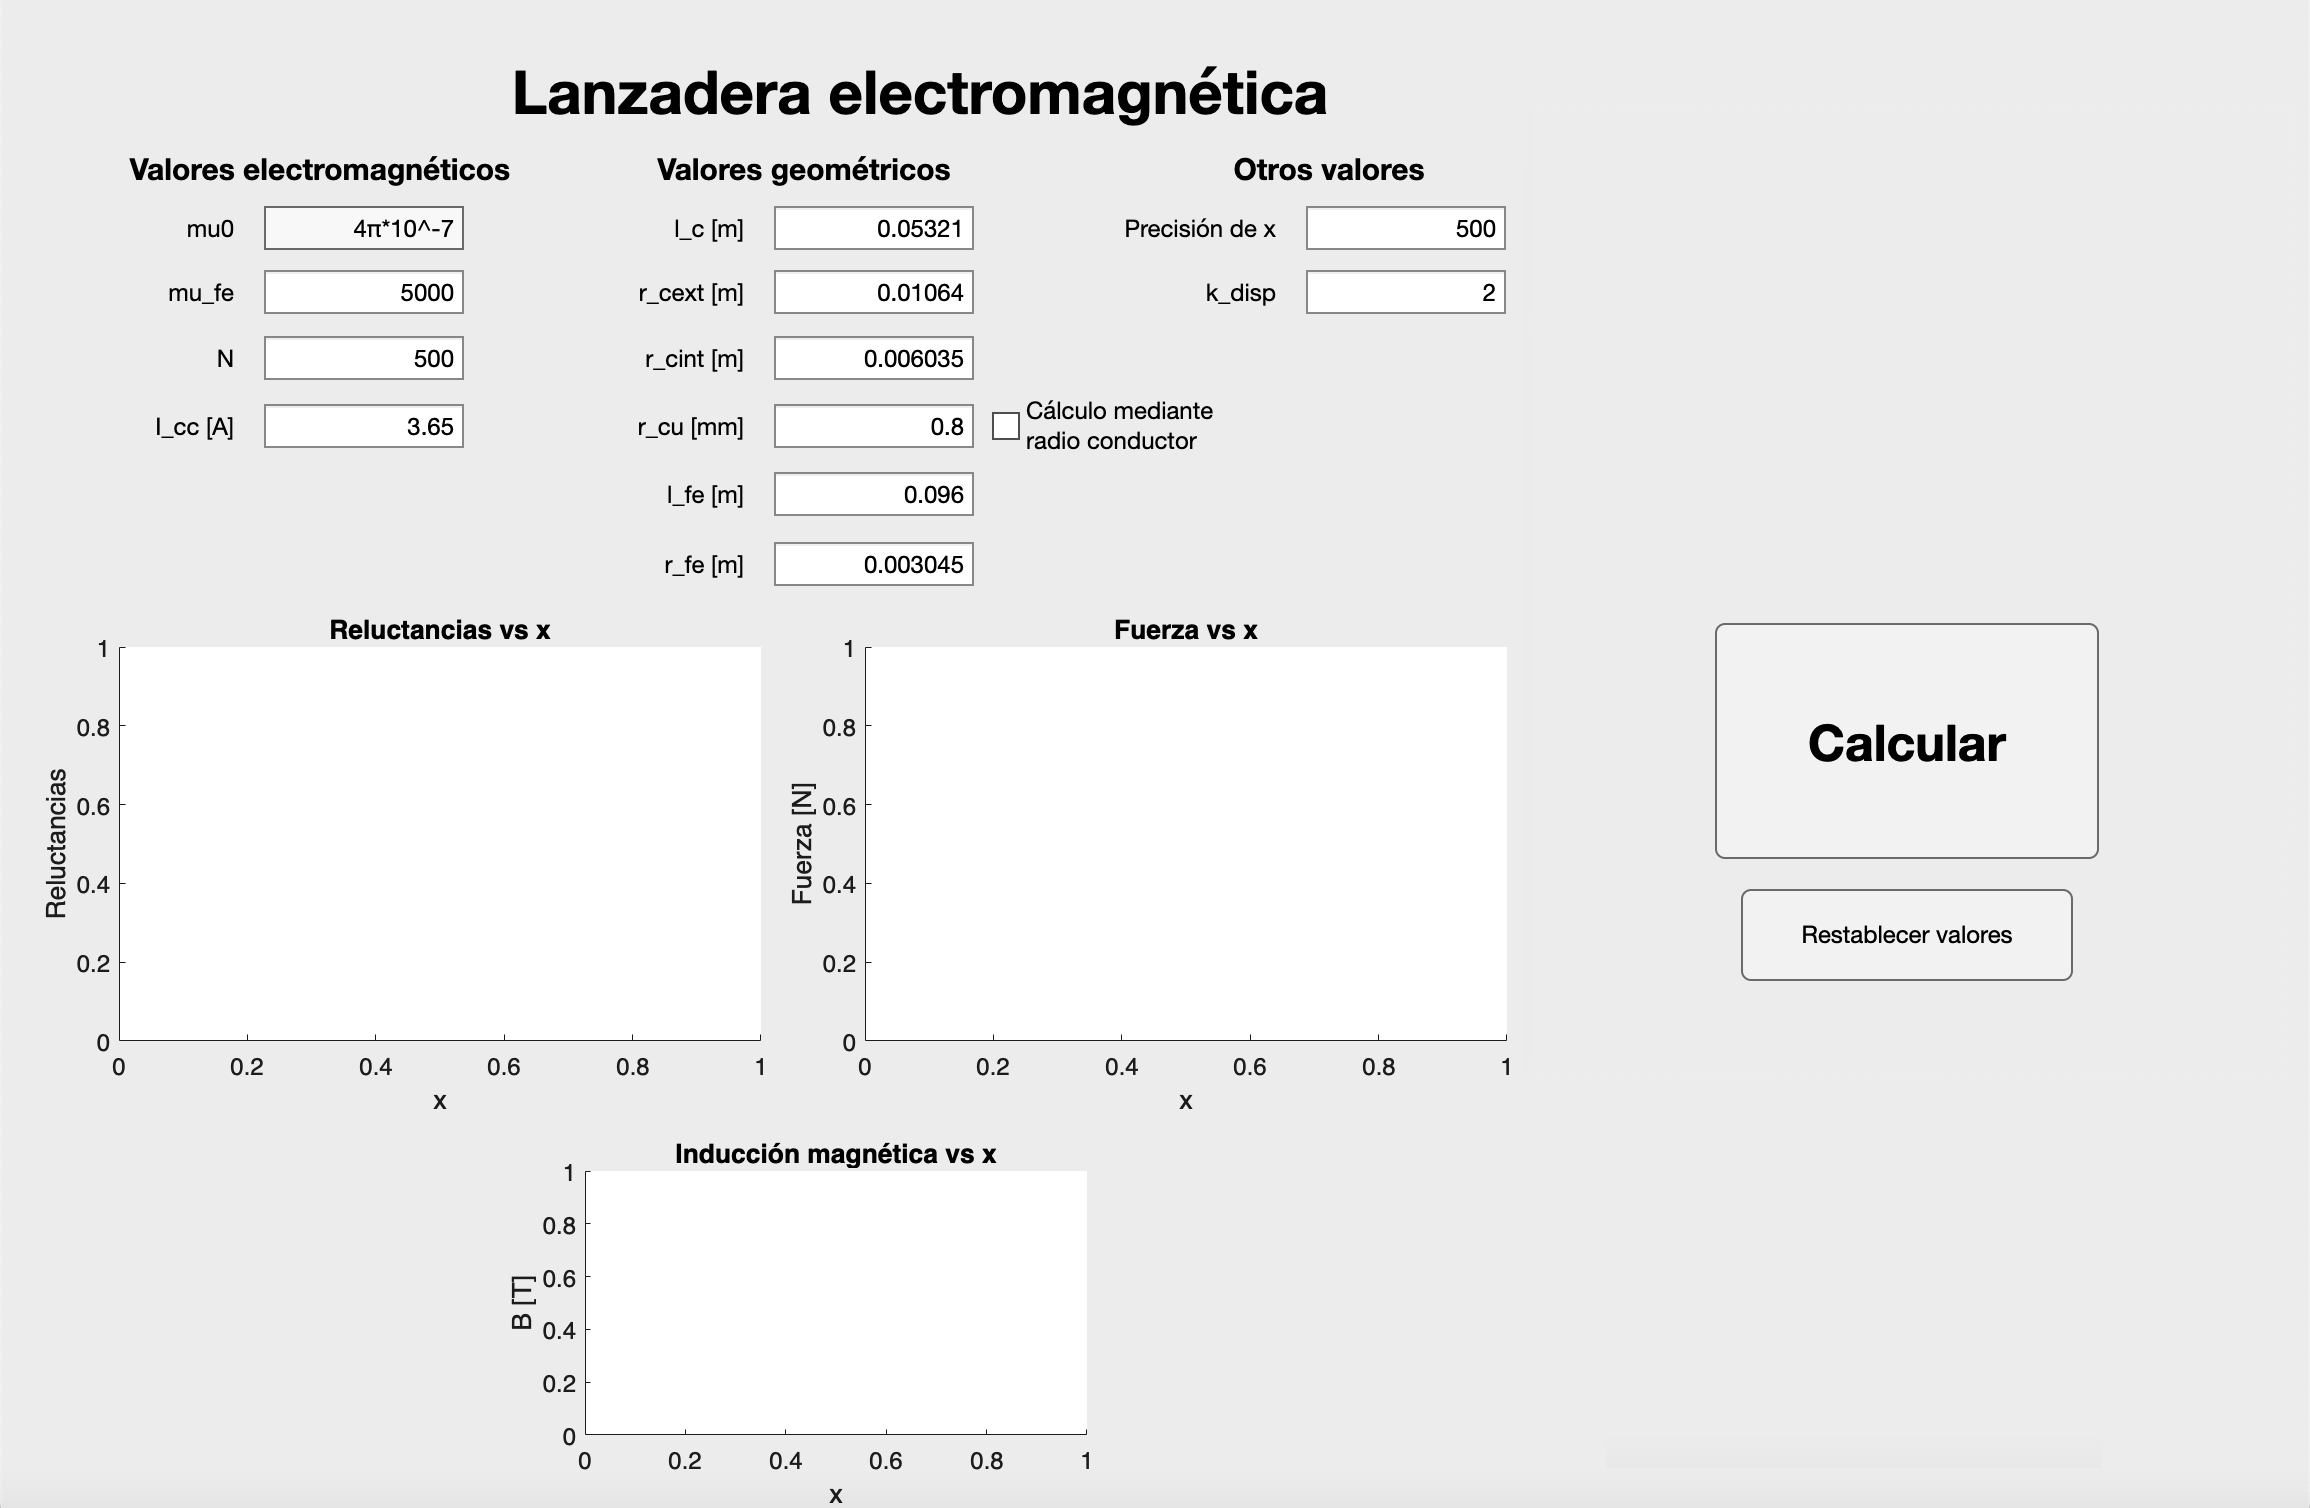
\includegraphics[width=7cm]{FigurasMemoria/calculadoraSinPista.png}
    \caption{Aplicación de ejemplo.}
    \label{fig:calculadoraSinPista} %Para referenciar -> \ref{fig:figNum}
\end{figure}

\newpage

\begin{figure}[H]
    \centering 
    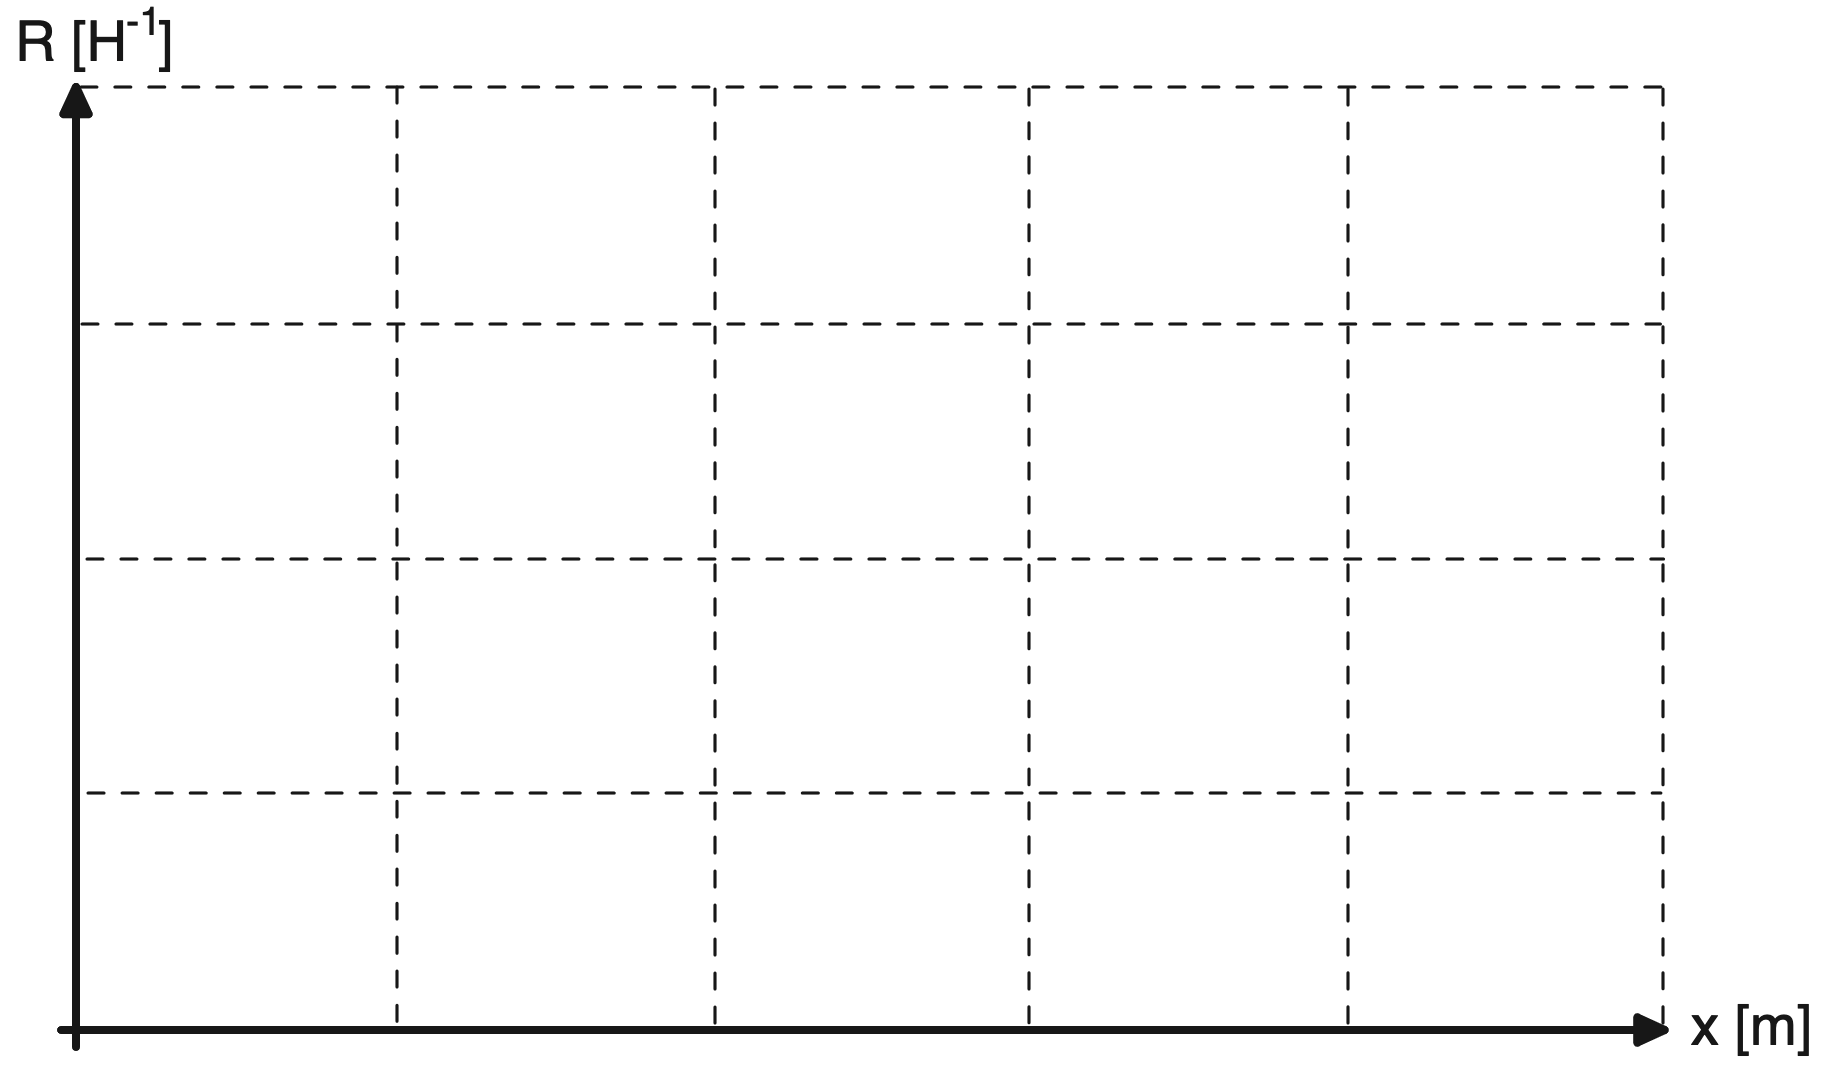
\includegraphics[width=0.75\textwidth]{FigurasMemoria/grafReluctPractica.png}
    \caption{Reluctancia en función de \textit{x}.}
    \label{fig:grafReluctPractica} %Para referenciar -> \ref{fig:figNum}
\end{figure}

\begin{figure}[H]
    \centering 
    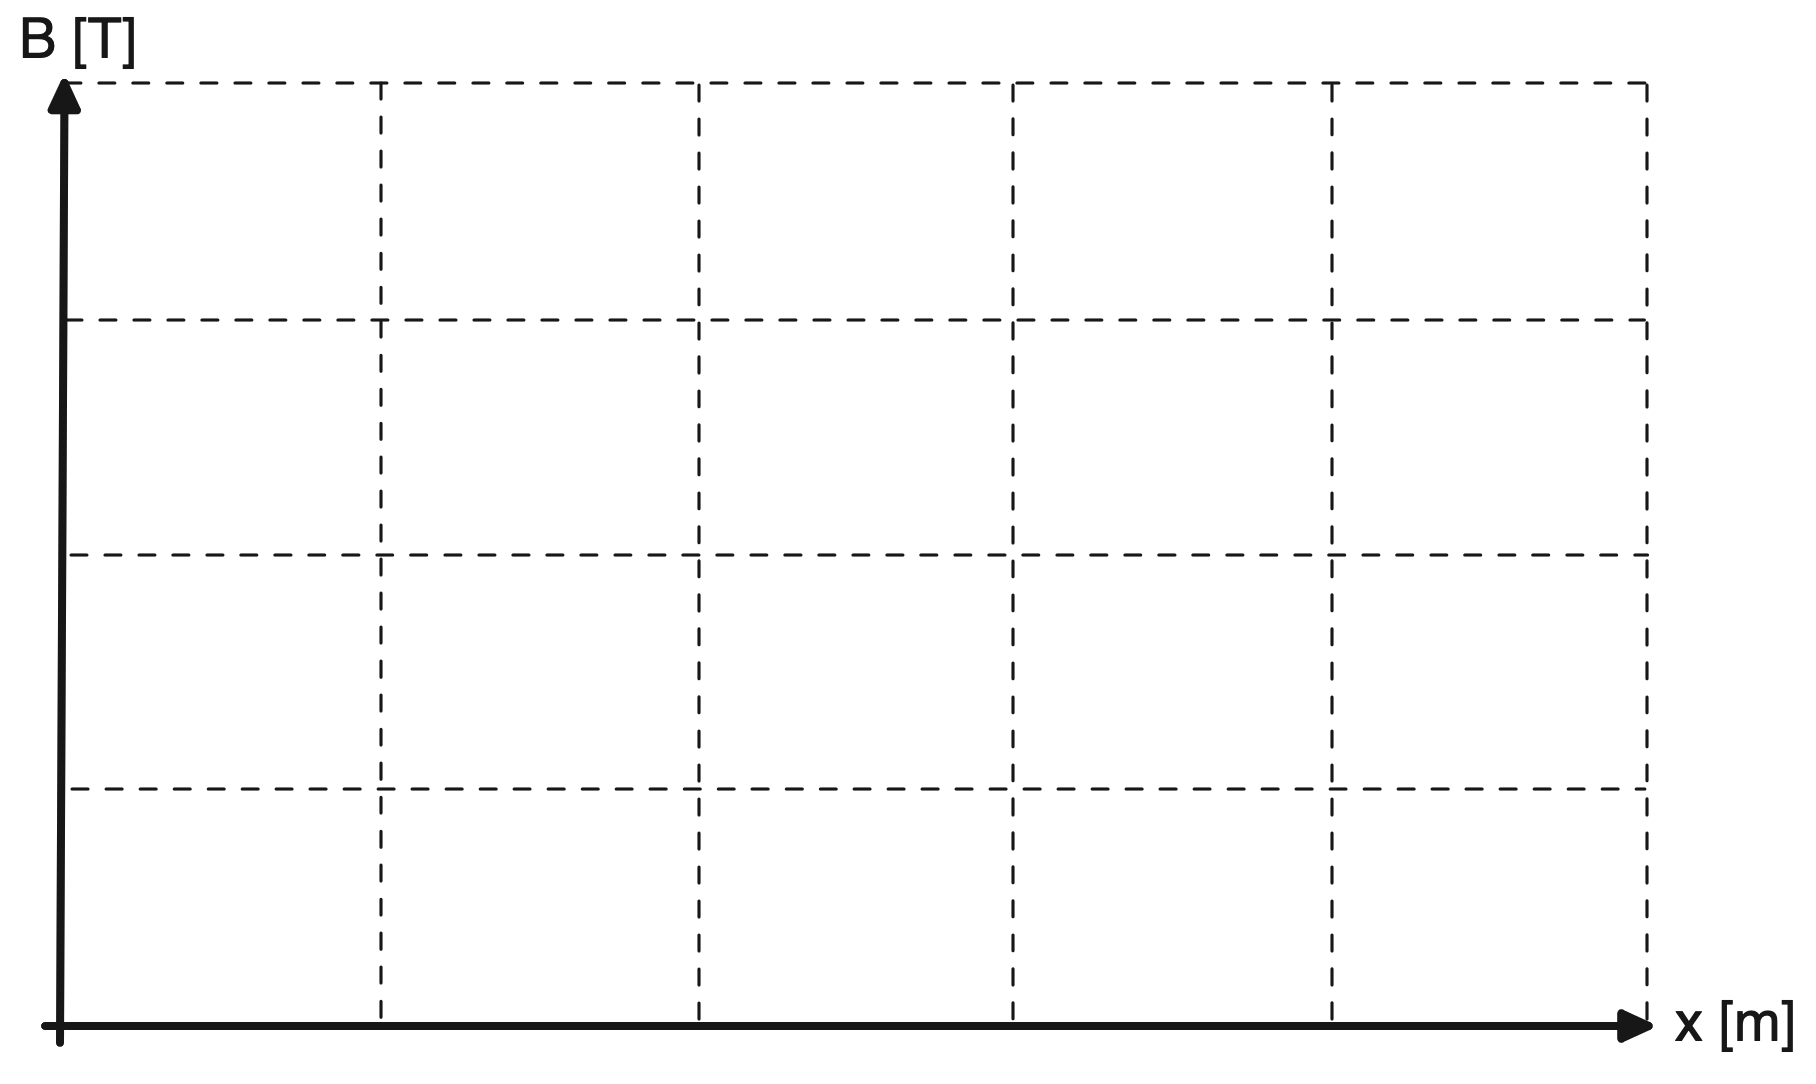
\includegraphics[width=0.75\textwidth]{FigurasMemoria/grafInducPractica.png}
    \caption{Inducción magnética en función de \textit{x}.}
    \label{fig:grafInducPractica} %Para referenciar -> \ref{fig:figNum}
\end{figure}

\begin{figure}[H]
    \centering 
    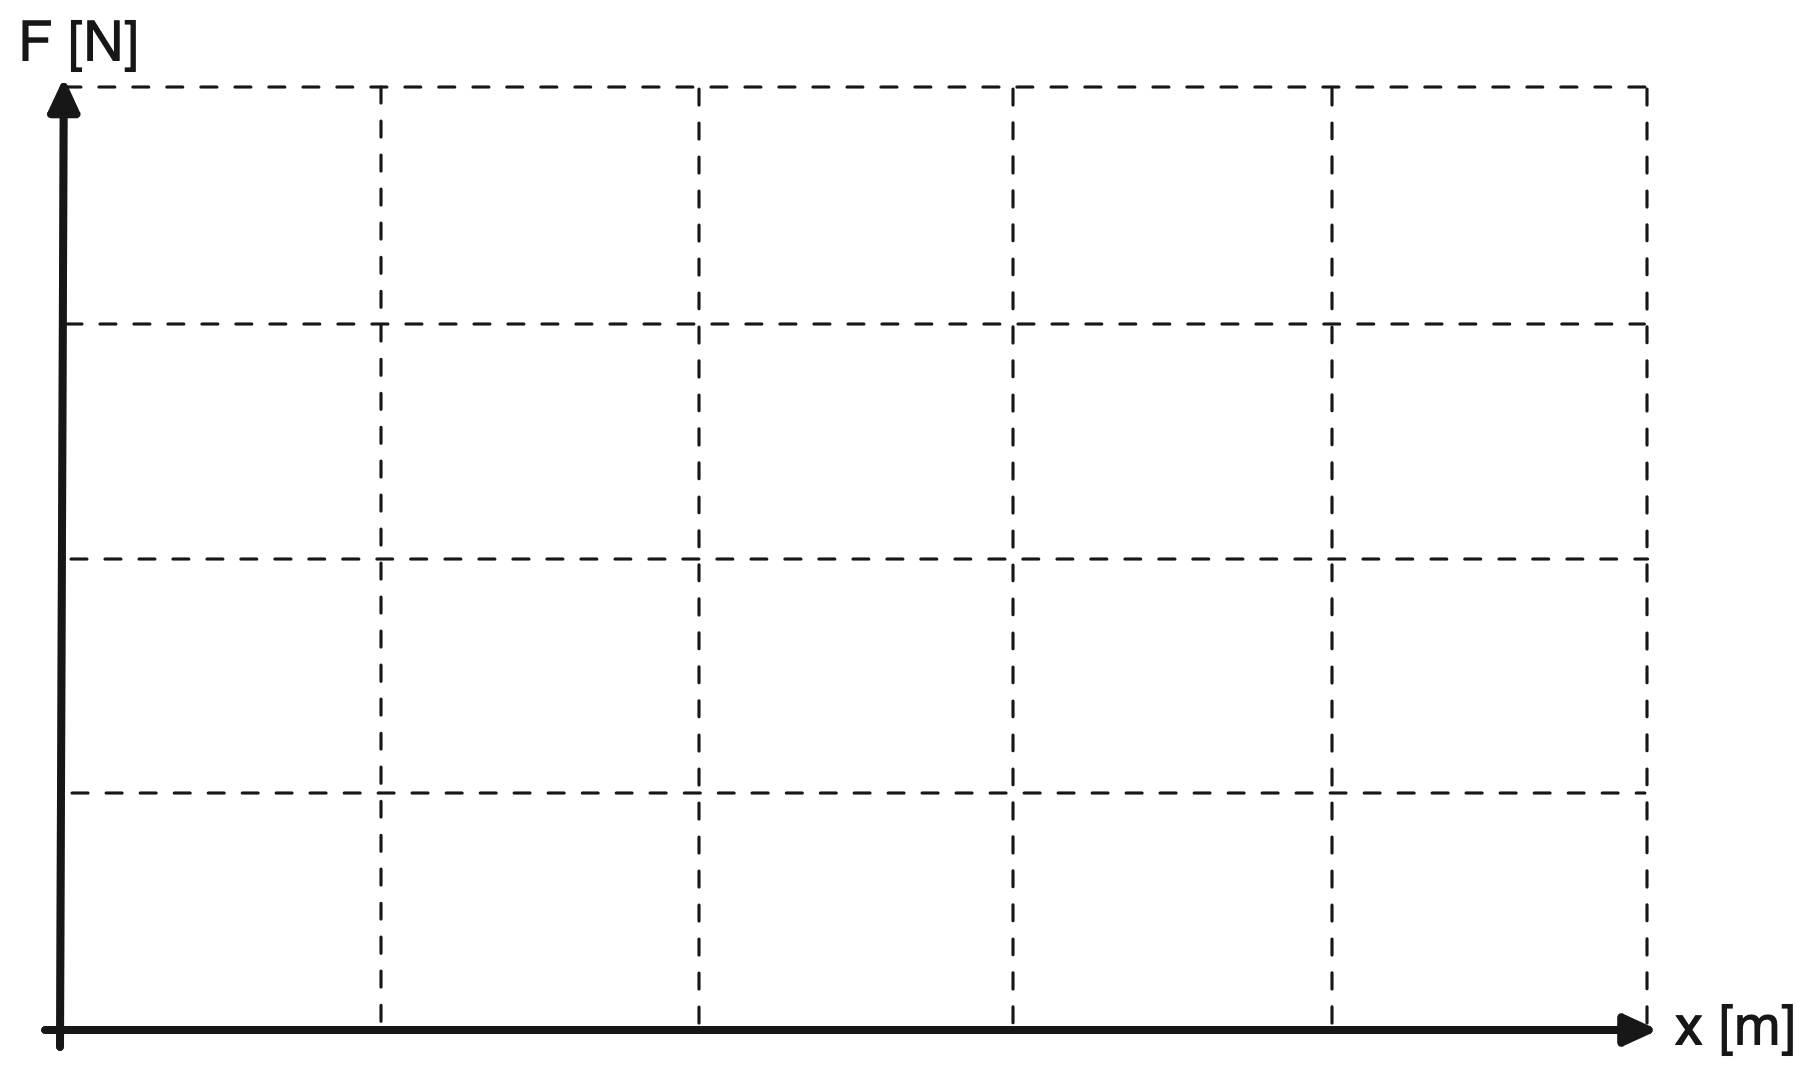
\includegraphics[width=0.75\textwidth]{FigurasMemoria/grafFuerzaPractica.png}
    \caption{Fuerza de atracción magnética en función de \textit{x}.}
    \label{fig:grafFuerzaPractica} %Para referenciar -> \ref{fig:figNum}
\end{figure}

\subsection*{Pruebas en el laboratorio}

En el laboratorio de electricidad se encuentra el \textit{banco de pruebas}, un montaje modular que nos permitirá tomar medidas de la fuerza y velocidad de la bobina.

\begin{figure}[H]
    \centering
    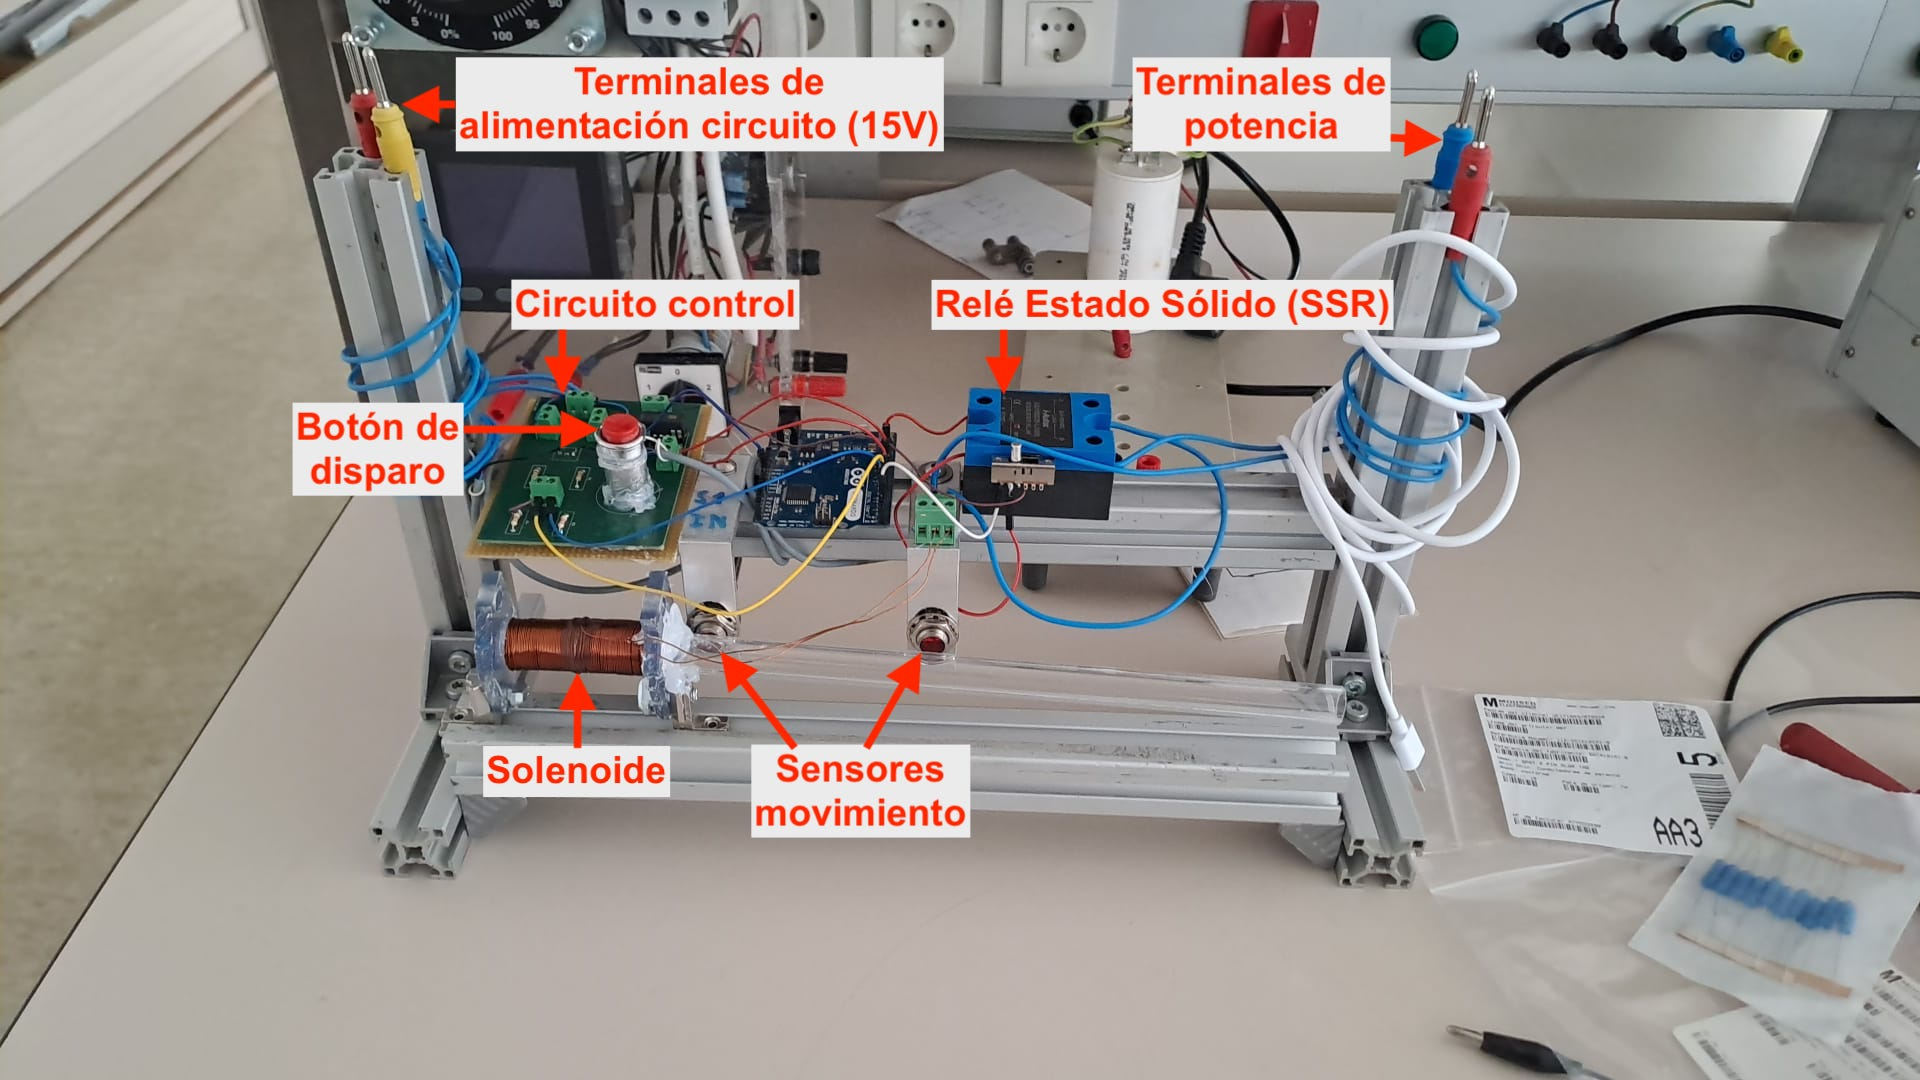
\includegraphics[width=10cm]{FigurasMemoria/prototipoFinalPractica.jpg}
    \caption{Banco de pruebas.}
    \label{fig:prototipoFinalPractica} %Para referenciar -> \ref{fig:figNum}
\end{figure}

El objetivo esta sección de la práctica es validar los modelos teóricos realizados anteriormente mediante la construcción y prueba de el solenoide de la \ref{tab:bobIniPractica}. Los medios para conseguir esto será emplear montaje de la figura \ref{fig:prototipoFinalPractica}, el cual cuenta con un circuito electrónico que controla los disparos de la bobina así como las mediciones de velocidad del vástago. Las medidas de fuerza se tomarán mediante el uso del dinamómetro.

Para realizar las mediciones de velocidad, habrá que seguir los siguientes pasos:

\begin{enumerate}
    \item Bobinar el solenoide sobre el cilindro escogido en el apartado 1 de la práctica.
    \item Comprobar que el valor \(r_{cext}\) no difiere mucho del calculado analíticamente. Si es así introducir el valor experimental de \(r_{cext}\) en la calculadora.
    \item Acoplar el solenoide al banco de pruebas.
    \item Asegurar que hay un sensor de movimiento justo en la salida del solenoide.
    \item Asegurar que el switch acoplado al relé de estado sólido cierra el circuito en el PIN2 del arduino.
    \item Alimentar el sistema:
    \begin{enumerate}
        \item Conectar el circuito eléctronico (terminales de la izquierda) a una tensión de 15 VDC.
        \item Conectar el arduino a un PC o portátil.
        \item Conectar los terminales del relé de estado sólido (terminales de la derecha) a la tensión \(V_{cc}\).
    \end{enumerate}
    \item Abrir el IDE de arduino.
    \item Acceder al repositorio \href{URL}{github.com/promerogomb/Codigo-Control-Lanzadera/} y descargar el código.
    \item Subir el código a la placa Arduino.
    \item Abrir el \textit{Serial Plotter}.
    \item Colocar el vástago al borde de la bobina.
    \item Pulsar el botón rojo.
    \item Observar la diferencia temporal en el \textit{Serial}.
\end{enumerate}

Una vez obtenida la diferencia temporal, se deberá medir la distancia entre los centros de los sensores para poder completar los cálculos siguiendo el siguiente procedimiento. El primer paso será calcular la velocidad de salida:

\[v_{vas}=\frac{d_{sens}}{\Delta t}\]

Conocida la velocidad, podemos calcular la aceleración a partir de la fórmula de la distancia recorrida para un movimiento rectilíneo uniformemente acelerado (con \(v_0 = 0~\text{ms}^{-1}\)):

\[d = v_0 * \Delta t + \frac{1}{2}*a*(\Delta t)^2 \rightarrow a = \frac{2d}{(\Delta t)^2}\]

Y desde aquí podemos obtener el valor de la fuerza según la segunda ley de Newton:

\[F=m*a\]

Una vez presentados ambos procedimientos, se pide rellenar la siguiente tabla:

\begin{table}[H]
    \centering
    \begin{adjustbox}{max width=\textwidth,center}
        \begin{tabular}{|c|c|c|c|c|c|}
        \hline
        \textbf{Distancia} & \textbf{Tiempo} & \textbf{Velocidad} & \textbf{Aceleración} & \textbf{Fuerza} & \textbf{Fuerza calculadora} \\
          &  &  &  &  &  \\
          &  &  &  &  &  \\
        \hline
        \end{tabular}
    \end{adjustbox}
    \caption{Resultados finales.}
    \label{tab:resultadosFinales}
\end{table}


\subsection*{Ejercicios adicionales}

Se plantean a continuación una serie de ejercicios y cuestiones adicionales para asegurar la comprensión completa de la práctica.

\subsubsection*{Conceptos}

\begin{itemize}
    \item ¿Cuáles son las ecuaciones de Maxwell relevantes para esta práctica y qué representan?
    \vspace{3cm}
    \item ¿Cómo es el valor de \(B\) en los extremos del solenoide frente a su centro? ¿Y la forma del campo?
    \vspace{3cm}
    \item Define con tus propias palabras lo que expresan las distintas ecuaciones de Maxwell:
    \begin{itemize}
        \item \(\vec{\nabla}\cdot \vec{E}= \frac{\rho}{\epsilon_0}\):
        \vspace{1cm}
        \item \(\vec{\nabla}\cdot \vec{B}=0\): 
        \vspace{1cm}
        \item \(\vec{\nabla}\times\vec{E}=-\frac{\partial\vec{B}}{\partial t}\):
        \vspace{1cm}
        \item:\(\vec{\nabla}\times \vec{B}=\mu_0\vec{J}+\mu_0\epsilon_0\frac{\partial \vec{E}}{\partial t}\):
        \vspace{1cm}
    \end{itemize}
\end{itemize}

\subsubsection*{Variaciones de parámetros}

\begin{itemize}
    \item ¿Por qué se analiza solamente el valor de la fuerza de atracción en \(x \in [0, l_c]\)?
    \vspace{2cm}
    \item Describe de manera justificada pero cualitativa lo que ocurre con la fuerza de atracción magnética al realizar las siguientes variaciones en algunos de los parámetros del solenoide:
    \begin{itemize}
        \item Aumentamos \(l_c\):
        \item Aumentamos \(N\):
        \item Disminuimos \(r_{fe}\):
        \item Disminuimos \(r_{cu}\):
    \end{itemize}
    \item Elige una nueva configuración geométrica para la bobina, simúlala en tu modelo de MATLAB\textsuperscript{\textregistered}, compárala con los resultados de la figura \ref{fig:grafFuerzaPractica} y discute la razón de la variación en el resultado. Los valores elegidos deben seguir respetando las restricciones impuestas.
    
    \begin{table}[H]
        \centering
        \setlength{\tabcolsep}{5pt}
        \renewcommand{\arraystretch}{1.2}
        \begin{tabular}{|c|c|c|c|c|c|c|}
            \hline
            \hbox{} & \textbf{\(D_{cu}\) [m]} & \textbf{\(r_{cint}\) [m]} & \textbf{\(l_c\) [m]} & \textbf{\(r_{fe}\) [m]} & \textbf{\(l_{fe}\) [m]} & \textbf{N} \\
            \hline
            \textbf{Valor inicial} &  &  &  &  &  &  \\
            \hline
            \textbf{Valor nuevo} &  &  &  &  &  &  \\
            \hline
        \end{tabular}
        \caption{Valores iniciales para la bobina de la lanzadera.}
        \label{tab:bobIniPractica2}
    \end{table}

    \begin{figure}[H]
        \centering 
        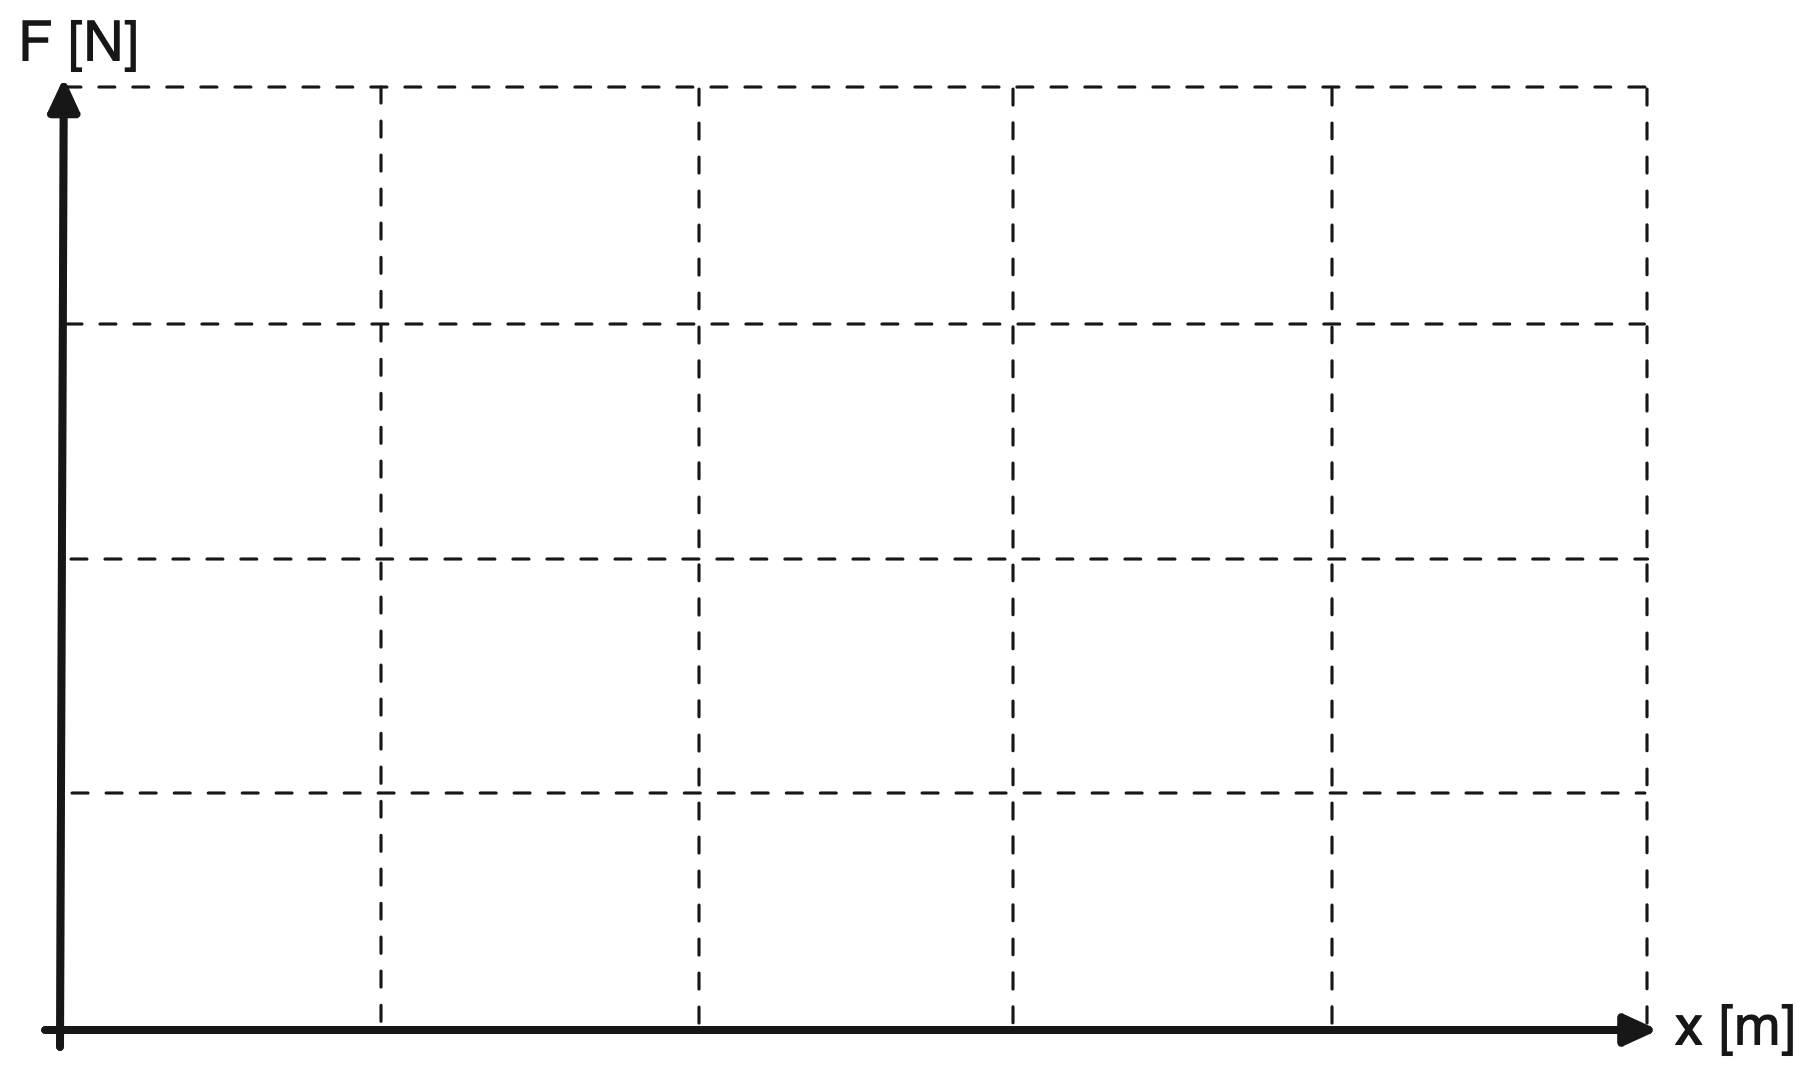
\includegraphics[width=0.75\textwidth]{FigurasMemoria/grafFuerzaPractica.png}
        \caption{Comparación de fuerzas.}
        \label{fig:grafFuerzaPracticaEjercicio} %Para referenciar -> \ref{fig:figNum}
    \end{figure}
    
\end{itemize}


